\section{Stability Analysis}

With regards to the stability analysis, we aim to try and prove some results on
the "stability function" $R(z)$ as seen in Levecue's \cite{levecue} chapter five
through eight and in Staff \cite{staff}. We heavily follow the arguments in
these sources to derive such results.

Suppose we have the following ordinary differential equation:
\begin{equation} \label{eq:lode}
  \begin{cases}
    u' = \mu u, \quad \mu < 0, t > 0 \\
    u(0) = u_0
  \end{cases}
\end{equation}
We would like to analyze the stability of parareal on this system with a 
course operator $\course$ and a fine operator $\fine$.

\subsection{A stability function $\mid$ Inspired by Euler Methods}

First we restrict ourselves to the infamous explicit and implicit Euler, with
the hope of deriving some stability criteria for them. Recall, that the explicit
and implicit euler scheme is:

\begin{align*}
  u_{n+1} & = u_n + \mu\Delta t u_n = (1 + \mu \Delta t)u_n & \text{ (Explicit
    Euler)} \\
  u_{n+1} & = u_n + \mu\Delta t u_{n+1} = (1 - \mu \Delta t)^{-1}u_n & \text{
    (Implicit Euler)} \\
\end{align*}

It's easy to see, after unrolling the recurrence on $u_n$, that these translate
to $u_{n+1} = (1+ \mu\Delta t)^n u_0$ or $(1 - \mu\Delta t)^{-n}$ for explicit
and implicit Euler respectively. Calling $R_e(z) = 1 + z$ and $R_i(z) =
(1-z)^{-1}$, we can analyze the stability of the method through these,
specifically we desire that $\abs{R(z)} \leq 1$, so that $R(z)^n$ doesn't blow
up in $n$.

With respect to Parareal, let's try and write our iteration in the form
$\lambda_n^k = H(n,k)\lambda_0$. Applying the explicit Euler iteration to
\ref{eq:parareal}, we see that it goes to:
\begin{align*}
  \lambda_{n+1}^{k+1} & = \course(t^{n+1},t^n,\lambda_n^{k+1}) +
  \fine(t^{n+1},t^n,\lambda_n^k) -
  \course(t^{n+1},t^n,\lambda_n^k) \\
  & = R_e(\mu\Delta t)\lambda_n^{k+1} + 
  R_e(\mu\delta t)^s \lambda_n^k -
  R_e(\mu\Delta t)\lambda_n^k \\
\end{align*}
where we say $s = \Delta t/ \delta t$, i.e. how many fine steps are needed to
make one course step. Combining like terms results in:
\[
  \lambda_{n+1}^{k+1} = 
  R_e(\mu\Delta t)\lambda_n^{k+1} + 
  \left( R_e(\mu\delta t)^s - R_e(\mu\Delta t)\right) \lambda_n^k 
\]
Now, if we were to note the terms on $\lambda$, we note that we have something
very similar to the recurrence relation on combinations $\binom{n}{k} =
\binom{n}{k-1} + \binom{n-1}{k-1}$. Exploiting that relationship, we can unroll
our recursion into:
\[
  \lambda_{n+1}^{k+1} = \left( \sum_{i=0}^k \binom{n}{i} \left[R_e(\mu \delta t)^s -
    R_e(\mu \Delta t)\right]^i R_e(\mu \Delta t)^{n-i} \right) \lambda_0 =
    H_e(\mu, n,k,\delta t, \Delta t) \lambda_0
\]
In doing this, we notice that any method for which we could write as $u_{n+1} =
R(z) u_n$ will have a very similar stability region, with $R_e \to R$. See
figure \ref{fig:stability} for the regions of stability under the Forward Euler
method.

\begin{figure}[!htb]
  \centering
  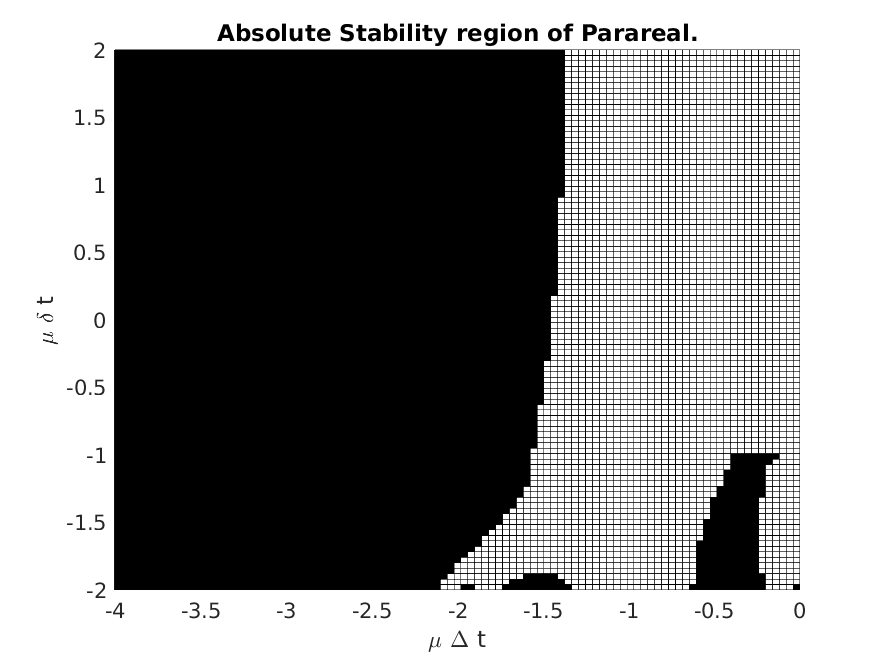
\includegraphics[width=.8\textwidth]{./resources/stability_fw}
  \caption{}\label{fig:stability}
\end{figure}
